\subsection{Repräsentativer Anwendungsfall für die Energiewirtschaft}\label{usecase}

Die verschiedenen Werttreiber und Anforderungen für ein Digitalisierungskonzept unterscheiden sich je nach Unternehmen und Branche.
Für eine erfolgreiche Transformation müssen daher individuelle Anwendungsfälle identifiziert werden.
In Anbetracht der Dynamik und des rasanten Tempos, in der neue Technologien entstehen,
ermöglicht ein anwendungsfallbasierter Ansatz eine flexible und agile Anpassung. \citep[S. 31]{Acharya2019}
\\Aus diesen Gründen wird im Folgenden ein repräsentativer Anwendungsfall für die Energiebranche vorgestellt. Die Anforderungen an das Zielsystem werden nach den von \citet{Lauenroth2016} vorgestellten Methoden erhoben.

\subsubsection{Ausgangsszenario} \label{usecase}

Der Windenergieanlagenhersteller Enercon GmbH aus Aurich verzeichnet 29000 Anlagen in 45 Ländern. Da das Kerngeschäft des Unternehmens auf den Bau von Anlagen für die dezentrale Energieerzeugung basiert, hat Industrie-4.0-Fähigkeit einen besonderen Stellenwert. Sei es die Einspeisung der produzierten Energie in das Smart-Grid, die Fernsteuerung oder die Zustandsüberwachung der Anlagen und Windparks: Das unternehmenseigene \acf{scada}-System ist auf die Enercon-Anlagen abgestimmt bietet umfangreiche Lösungen für die Kunden. Allerdings versendet das \ac{scada}-System die Messwerte bisher nur alle 10 Minuten das \ac{cms}. Zudem ist es eine technische Insellösung, welche die betriebswirtschaftliche Welt nicht integriert. Als Kunden stehen die Energieversorgungsunternehmen im Vordergrund, mit denen Enercon Verträge für Wartungsservices abschließt. Die Enercon-IT nutzt SAP-Produkte für das Management der Ressourcen, Logistik oder Kunden. Im Zuge der Anpassung an die Anforderungen der digitalen Welt wird SAP jedoch den Support der bisher auch von Enercon verwendeten Standard-ERP-Software bis 2025 einstellen. Der Fokus wird auf das Nachfolgeprodukt SAP S/4 HANA gesetzt, welche die echtzeitfähige In-Memory-Datenbanktechnologie \acf{hana} für nutzt. Aus diesem Grund bereitet sich Enercon rechtzeitig auf die Migration auf S/4 HANA vor. Die Integrations- und Entwicklungsplattform von \ac{hana} bietet zahlreiche Möglichkeiten zur Realisierung von innovativen Softwarelösungen sowohl auf der Cloud als auch On-Premise. Die Neuausrichtung der IT-Architektur ist auch für die erfolgreiche digitale Transformation von Enercon großer Bedeutung.

\noindent Im besonderen Interesse liegt die SAP Leonardo \ac{iot} Foundation, vor allem in Anbetracht einer möglichen Integration von Stammdaten aus dem S/4 HANA System. Dafür ist zunächst eine Analyse der SAP Leonardo Systemarchitektur mitsamt der Perspektiven gewünscht. Dies könne als Entscheidungsgrundlage für eine Erweiterung des Geschäftsfeldes von Energieproduktion auf IT-Dienstleistungen dienen. Außerdem soll prototypisch dargestellt werden, inwiefern sich SAP Leonardo IoT als Verwaltungsschale für die Industrie-4.0-Komponente eignet. Langfristiges Ziel des Unternehmens sei es, das \ac{scada}-System echtzeitfähig zu gestalten. Um Risiken vor Inbetriebnahme und Kosten zu minimieren soll jedoch zunächst eine einfache Simulation genügen.

\noindent Die Simulation soll dem Servicepersonal in der Wartung und den Kunden ermöglichen, die Zustandsdaten des digitalen Zwillings einer Anlage in Echtzeit zu überwachen. Wenn kritische Messwerte empfangen werden, soll das Personal sofort benachrichtigt werden, damit Wartungsmaßnahmen eingeleitet werden können. Die Softwareentwickler/innen sollen den Prototypen beliebig sowohl um (Mess-)Geräte als auch um App-Funktionalitäten erweitern können.

\subsubsection{Anforderungserhebung}

Um die Anforderungen für die Umsetzung einer repräsentativen Lösung zu bestimmen, muss zunächst ermittelt werden, welche Einflussfaktoren sich im Kontext des Zielsystems befinden und wo sich die Grenze des Systems befindet. Mit der Evaluation der Ausgangssituation (s. \ref{usecase}) können Anforderungsquellen identifiziert werden, welche sich auf das Zielsystem beziehen und sich im Systemkontext befinden. Auf Grundlage der Evaluation werden zunächst Probleme, Anforderungen und Lösungen für das System definiert. Für eine bessere Strukturierung des Systems werden die einzelnen \ac{pal} auf die Ebenen System und Systemkontext, sowie auch auf die technische Ebene abstrahiert. Die Dokumentation von Anforderungen auf verschiedenen Abstraktionsebenen ist vor allem für die nachträgliche Verwaltung der Anforderungen für zukünftige Softwareprojekte von großem Wert \citep{Lauenroth2016}. Nach \citet{IREB2017} unterscheidet man typischerweise zwischen drei Arten von Anforderungen: funktionale Anforderungen, Qualitätsanforderungen sowie Randbedingungen.
Die Formulierung von Anforderungen setzt das Vorhandensein einer Lösung voraus, weshalb auch der Prototyp bereits als Anforderungsquelle gelten kann.
\\\\Aus der Evaluation der Ausgangssituation ergibt sich die in Abbildung \ref{kontext} dargestellte Systemabgrenzung. Die Anforderungsanalyse berücksichtigt die Stakeholder, welche sowohl mit dem System interagieren als auch direkten Einfluss auf die Anforderungen haben. Als Nutzer des Systems kristallisieren sich die Kunden Enercons (z.B. die \ac{evu}) sowie das Servicepersonal in der Wartung. Stakeholder mit qualitativen Anforderungen an das System sind die Softwareentwickler/innen und -architekt(inn)en, für welche der Prototyp als Architekturvorlage dienen soll. Die Auftraggeber stellen die direkte Anforderung, eine Lösung und Analyse für SAP Leonardo zu entwickeln, die die Eignung SAP Leonardos als Verwaltungsschale für die \ac{i40} beurteilt. Dies impliziert, dass sich an der IT-Sicht (s. Abbildung \ref{it_layer}) der Referenzarchitektur RAMI 4.0 und an dem Konzept der Industrie-4.0-Komponente (s. Abschnitt \ref{rami}) orientiert werden soll. Berücksichtigt werden sollen außerdem die Anforderungen, die sich aus der Beschaffenheit der Branche der Energiewirtschaft ergeben. Bereits existierende Systeme können ebenfalls Einfluss auf das System haben, was jedoch für die Prototypentwicklung nicht relevant ist.


\begin{figure}[h]
  \centering
  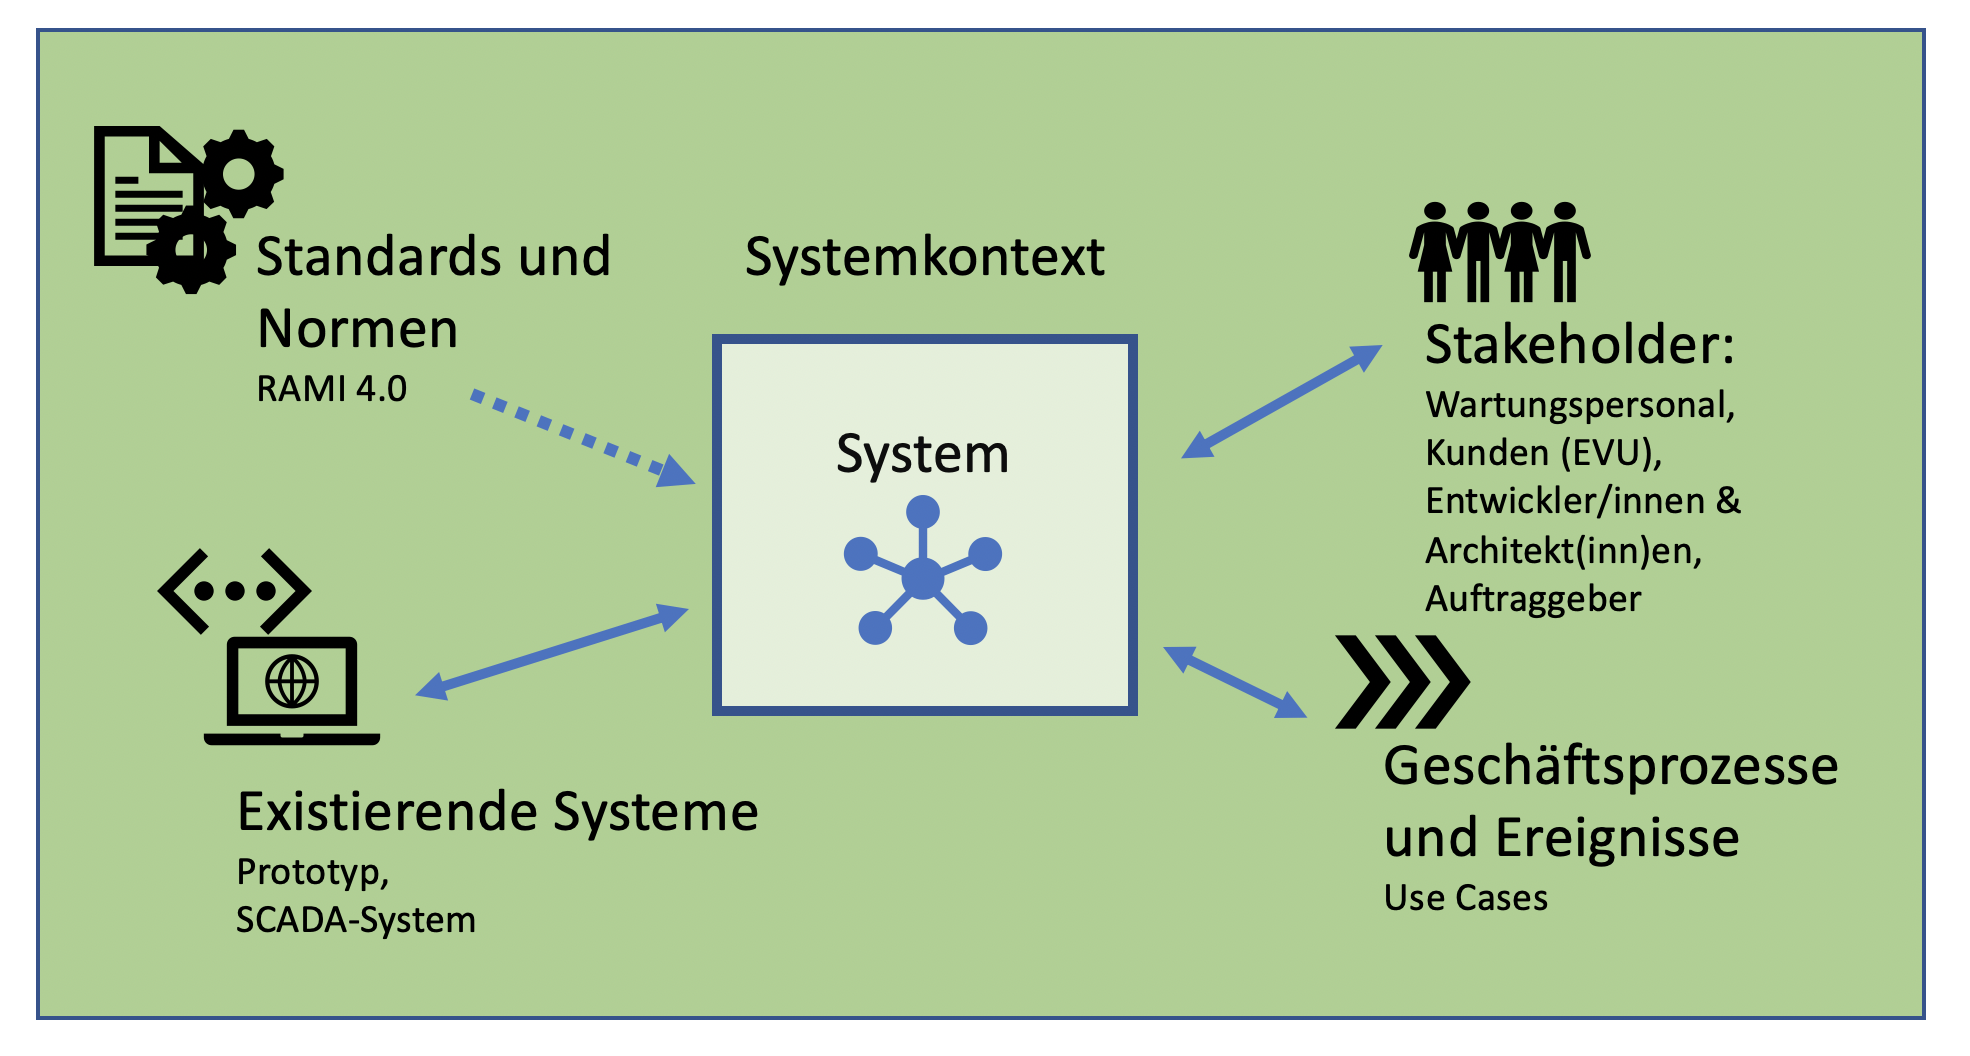
\includegraphics[width=1\linewidth]{System_Kontext.png}
  \caption[Systemabgrenzung und Systemkontext]{Systemabgrenzung und Systemkontext}
  \label{kontext}
\end{figure}

% Anforderungsanalyse ***********

\subsection{Anforderungsanalyse}
Im folgenden Kapitel wird die Anforderungsanalyse nach Abstraktionsebenen des \ac{pal}-Modells (s. Tabelle \ref{pal}) durchgeführt. In der Kontextebene werden Anforderungen bestimmt, welche sich direkt oder indirekt die Funktionen des Systems bestimmen. Die Behandlung der Forschungsfrage FF1.1, welche Anforderungen an ein System für die digitale Transformation sich aus Sicht der dezentralen Energieerzeugung ergeben, schafft die Grundlage für die Problemdefinition für die Funktionsweise des eigentlichen Systems. Die Funktionen werden in der Systemebene mit den notwendigen Schnittstellen und Datenstrukturen in einen logischen Aufbau eingeordnet. Anschließend wird auf der technischen Ebene der logische Aufbau technisch beschrieben.


\begin{table}[h]
  \begin{tabular}{ p{4cm}|p{5cm}|p{4cm} }
    \toprule
    Problem & Anforderung & Lösung \\
    \midrule
    \multicolumn{3}{ l }{\textbf{Kontextebene} }\\
    \hline
    K-P-N & K-A-N & K-L-N\\
    \hline
     \multicolumn{3}{ l }{\textbf{Systemebene} }\\
     \hline
     S-P-N & S-A-N  & S-L-N\\
  \hline
    \multicolumn{3}{ l }{\textbf{Technische Ebene} }\\
    \hline
    T-P-N & T-A-N  & T-L-N\\
    \bottomrule
    \end{tabular}
    \label{pal_table}
  \caption{Das PAL-Modell}
  \label{pal}
\end{table}

% Kontextebene
\subsubsection {Kontextebene}

\paragraph{Problemstellungen}
Die Probleme, die durch das Zielsystem gelöst werden sollen, sind durch verschiedene Einflussfaktoren aus dem Kontext des Systems verursacht. In erster Linie steht das Problem der dezentralen Energieerzeugung aus dem Branchenkontext (s. Abschnitt \ref{energy}). Da die Erzeugung von schwankenden (Umwelt-) Bedingungen abhängt, müssen kontinuierlich Daten erhoben werden, um Leistungsqualität und -verfügbarkeit zu gewährleisten. Gleichzeitig steigt der Koordinationsaufwand aufgrund der großen Datenmengen. Weil die \ac{scada}-Systeme Messdaten nur im 15-Minuten-Takt versenden, können keine aktuellen Zustandsdaten eingesehen und nicht rechtzeitig auf Probleme reagiert werden. Problematisch ist dies besonders in Anbetracht der erhöhten Steuerungskomplexität der Anlagen.
Als ein weiteres Problem kann die hohe Abhängigkeit der Branche von gesetzlichen Vorgaben gesehen werden. Die sich regelmäßig ändernden Regularien können die Strukturen und die Beschaffenheit der Branche grundlegend ändern. Aus diesem Grund kann sich die Umsetzung von ohnehin schon komplexen und interdisziplinären Industrie-4.0-Projekten für die Energiebranche als große Herausforderung erweisen, aber auch einen enormen Mehrwert bringen. Zudem ergibt sich aus dem Ausgangsszenario die Problematik, dass das bestehende System zur Zustandsüberwachung keine Integration von intelligenten Diensten ermöglicht. Mit dem Umstieg auf SAP S/4 HANA stellt sich die Frage, inwiefern sich das  Innovationsportfolio SAP Leonardo als Verwaltungsschale für die Anlagen eignet. In diesem Zusammenhang ergibt sich aus dem Ausgangsszenario jedoch die Problematik des erhöhten Risikos bei großen Industrie-4.0-Projekten. Auch \citet{Lauenroth2016} mahnen bei Projekten für Anlagen mit komplexer Systemelektronik und -mechanik zur Vorsicht. Ein Change Request für solch komplexe Systeme wie Windenergieanlagen wäre zu teuer.

\begin{table}[H]
  \begin{tabularx}{\textwidth}{@{}lXp{2cm}@{}}
      \toprule
      ID                & Problem & Quelle \\
      \midrule
      \textbf{K-P-1}              &       Anstieg der Steuerungskomplexität der Anlagen wegen der dezentralen Energieerzeugung               & \textit{Branche}                \\
      \multicolumn{1}{r}{K-P-1.1} &  Koordination großer Datenmengen     \\
      \multicolumn{1}{r}{K-P-1.2} &  Die Gewährleistung der Leistungsqualität und Leistungsverfügbarkeit \\
      \multicolumn{1}{r}{K-P-1.3} &  Verzögerung der Reaktion auf Probleme aufgrund des 10-Minuten-Takts der SCADA-Systeme & \textit{Auftraggeber} \\\addlinespace
      \textbf{K-P-2}              & Strenge Regularien können die Branche stetig ändern                     & \textit{Branche}                \\ \addlinespace
      \textbf{K-P-3}              & Interdisziplinäre und komplexe Struktur von Industrie-4.0-Projekten                      & \textit{RAMI 4.0}                \\
      \textbf{K-P-4}              &  Eignung der SAP Leonardo Foundation als Verwaltungsschale  & \textit{Auftraggeber} \\
      \multicolumn{1}{r}{K-P-4.1} &  Nutzung von intelligenten Diensten\\
      \multicolumn{1}{r}{K-P-4.2} &  Erhöhtes Risiko bei der Umsetzung großen Industrie-4.0-Projekte\\
      \addlinespace
      \bottomrule
  \end{tabularx}
  \label{kontext_probleme}
  \caption{Probleme aus Kontextebene}
\end{table}

\paragraph{Kontextmodell}

Die oben definierten Probleme schaffen eine Struktur für ihre Lösung (vgl. \ac{pal}-Modell Lösungssäule). Mit dem  Kontextmodell wird eine erste statische Struktur des Zielsystems auf Grundlage der identifizierten Anwendungsfälle und Lösungsmöglichkeiten geschaffen \citep{Lauenroth2016}. Als Nutzer des Systems bestimmen die Anwendungsfälle des Kunden und des Wartungspersonals die erste grobe Struktur des Systems, doch sie wird genau so durch die Rahmenbedingungen im Systemkontext geformt.
Mit dem in Abbildung \ref{usecase_basic} dargestellten Use Case Diagramm werden zusammenhängende Anwendungsfälle zur Lösung der Probleme in K-P-1 aufgeführt. In dem Diagramm wird der gewünschte Geschäftsprozess des Auftraggebers für die Nutzer in Elemente aufgeteilt, die durch das System aufgegriffen werden.

\begin{figure}[ht]
  \centering
  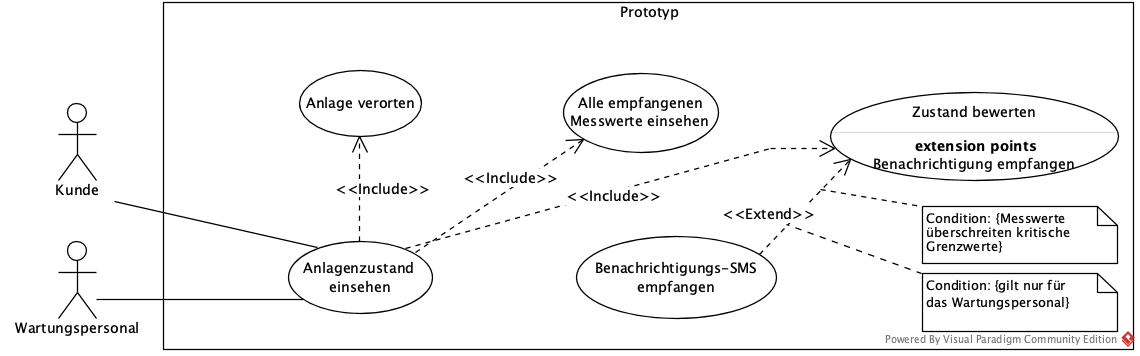
\includegraphics[width=1.0\linewidth]{use_case_basic.png}
  \caption[Use Case Diagramm der Kontextebene]{Use Case Diagramm der Kontextebene}
  \label{usecase_basic}
\end{figure}


\noindent Gelöst werden die Probleme jedoch in erster Linie durch die Verfügbarkeit einer intelligenten Verwaltungsschale über der physischen Anlage nach dem Konzept der Industrie-4.0-Komponente (s. Abschnitt \ref{rami}).
Ein wesentliches Merkmal von Industrie"=4.0"=Projekten ist die Interdisziplinarität und Komplexität (K-P-3). Für den Aufbau einer Strategie und die Bewältigung der Herausforderungen, die ein komplexes System stellt, wird eine von Politik und Wirtschaft entwickelte Referenzarchitektur als Hilfe herangezogen. Das \ac{rami} bildet (s. Abschnitt \ref{rami}) eine wichtige Entscheidungsgrundlage für die Beurteilung der Eignung (K-P-4) der prototypischen Architektur eines solchen Systems. Da die Umsetzungsstrategie der Plattform Industrie 4.0 \citep{BITKOM2015} erneuerbare Energien nicht berücksichtigt, aber die Abhängigkeit von fluktuierenden Regularien (K-P-2) besteht, soll eine unternehmensspezifische Architekturvorlage entwickelt werden.


\paragraph{Anforderungen}

Die Anforderungsdefinition in der Kontextebene ist von hoher Abstraktion geprägt. Sie entstehen aus den wesentlichen Problemen, die das Zielsystem zu lösen hat. Es wird zunächst ein grober Überblick über die wichtigsten Anforderungen an das Gesamtsystem gegeben, um eine Orientierung für die Anforderungserhebung auf Systemebene zu schaffen. Nach \citet{Doleski2016} gibt es drei wesentliche Herausforderungen für Energieunternehmen. Zum einen gilt es die Informationsflut aus der dezentralen Produktion zu bewältigen. Bezogen auf das Zielsystem bedeutet dies, Messwerte aus der Anlage in einem digitalen Zwilling visuell bereitzustellen. Außerdem müssen diese Informationen Wissen erzeugen. Das System muss dies durch die Bereitstellung von prädiktiven Informationen und durch Reaktion auf kritische Zustände ermöglichen. Zudem müssen aus den Informationen relevante Erkenntnisse für die Unternehmensführung gewonnen werden. Dafür muss das Zielsystem eine Möglichkeit für die Einbindung von intelligenten Diensten zur Datenverarbeitung aufweisen. Für einen besseren Überblick sind die Anforderungen im Anhang  \ref{anfkontext} gelistet.


\subsubsection{Systemebene}
Um den inneren logischen Aufbau Prototypen zu spezifizieren, müssen die Lösungen und Anforderungen der Kontextebene erneut in zu lösende Probleme zerlegt werden. Anschließend wird das Systemmodell vorgestellt, welches mit seinen Schnittstellen, Funktionen und Datenstrukturen die Probleme lösen soll. Da aus der Spezifikation der Systemfunktionen sich neue Anwendungsfälle ergeben, werden diese ebenfalls spezifiziert. Schließlich werden die Anforderungen an das System definiert.

\paragraph{Problemstellungen} Damit der Prototyp die Anforderungen der des Systemkontextes lösen kann, muss es spezielle Probleme lösen. Das Hauptproblem ist die Virtualisierung eines physischen Assets mitsamt der zugehörigen Messdaten. Unabhängig davon, wo sich der Nutzer befindet, soll er jederzeit den Zustand der Anlage durch den digitalen Zwilling einsehen können. Dabei soll es dem Nutzer ermöglicht werden, den digitalen Zwilling eindeutig einer realen Anlage zuzuordnen. Um einen Mehrwert aus den gemessenen Daten zu erlangen, muss der Prototyp die Bedeutung bestimmter Daten erkennen und ggf. eine Benachrichtigung versenden.

\begin{table}[ht!]
  \begin{tabularx}{\textwidth}{@{}lXp{2cm}@{}}
      \toprule
      ID                & Problem & Quelle \\
      \midrule
      \textbf{S-P-1}              &       Übergabe des physischen Assets in die digitale Welt               & \textit{K-FA-1}                \\
      \multicolumn{1}{r}{S-P-1.1} &  Empfang aller Zustandsdaten der Anlage     \\
      \multicolumn{1}{r}{S-P-1.2} &  Identifikation der Anlage     \\
      \multicolumn{1}{r}{S-P-1.3} &  Erkennung der Bedeutung eines Messwerts  & \textit{K-FA-1.3}\\
      \multicolumn{1}{r}{S-P-1.4} &  Orts- und zeitunabhängige Anzeige der Zustandsdaten einer Anlage     \\
      \multicolumn{1}{r}{S-P-1.5} &  Verortung einer Anlage & \textit{K-FA.1.2}\\
      \multicolumn{1}{r}{S-P-1.6} &  Erkennung der Grenzüberschreitung eines Messwerts & \textit{K-FA-1.4}\\
      \multicolumn{1}{r}{S-P1.7} &  Erkennung der Notwendigkeit einer erneuten Benachrichtigung\\
      \textbf{S-P-2}              &  Bereitstellung einer flexiblen Systemarchitektur  & \textit{K-QA} \\
      \textbf{S-P-3}              &  Bereitstellung einer standard-konformen Systemarchitektur & \textit{K-RA} \\
      \addlinespace
      \bottomrule
  \end{tabularx}
  \label{system_probleme}
  \caption{Probleme aus Systemebene}

\end{table}


\paragraph{Systemmodell}

Damit der Prototyp die Anwendungsfälle aus Abbildung \ref{usecase_basic} ermöglichen kann, enthält es im Inneren bestimmte Funktionen, Schnittstellen und Datenstrukturen. Von der Virtualisierung der Anlage bis zur Präsentation für den Nutzer fließen viele Daten. Der Fluss der Daten über die Funktionen und Schnittstellen ergibt ein erstes grobes Systemmodell (s. Abbildung \ref{dataflow}). Die gelben Objekte repräsentieren sind Schnittstellen\footnote{Die Notation ist an das Datenflussdiagramm angelehnt, wobei die Darstellung leicht verändert wurde.}, die die Verbindung des Systems mit der Umwelt beschreiben. Über die Funktionen (grün) fließen die Daten an die Datenspeicher (rot), bis sie schließlich bei den Nutzern ankommen. Dieses Diagramm dient nicht dazu, den Datenfluss zu kontrollieren, d.h. Bedingungen zu setzen. Es soll lediglich einen Überblick über den Aufbau des Systems geben.

\begin{figure}[ht!]
  \centering
  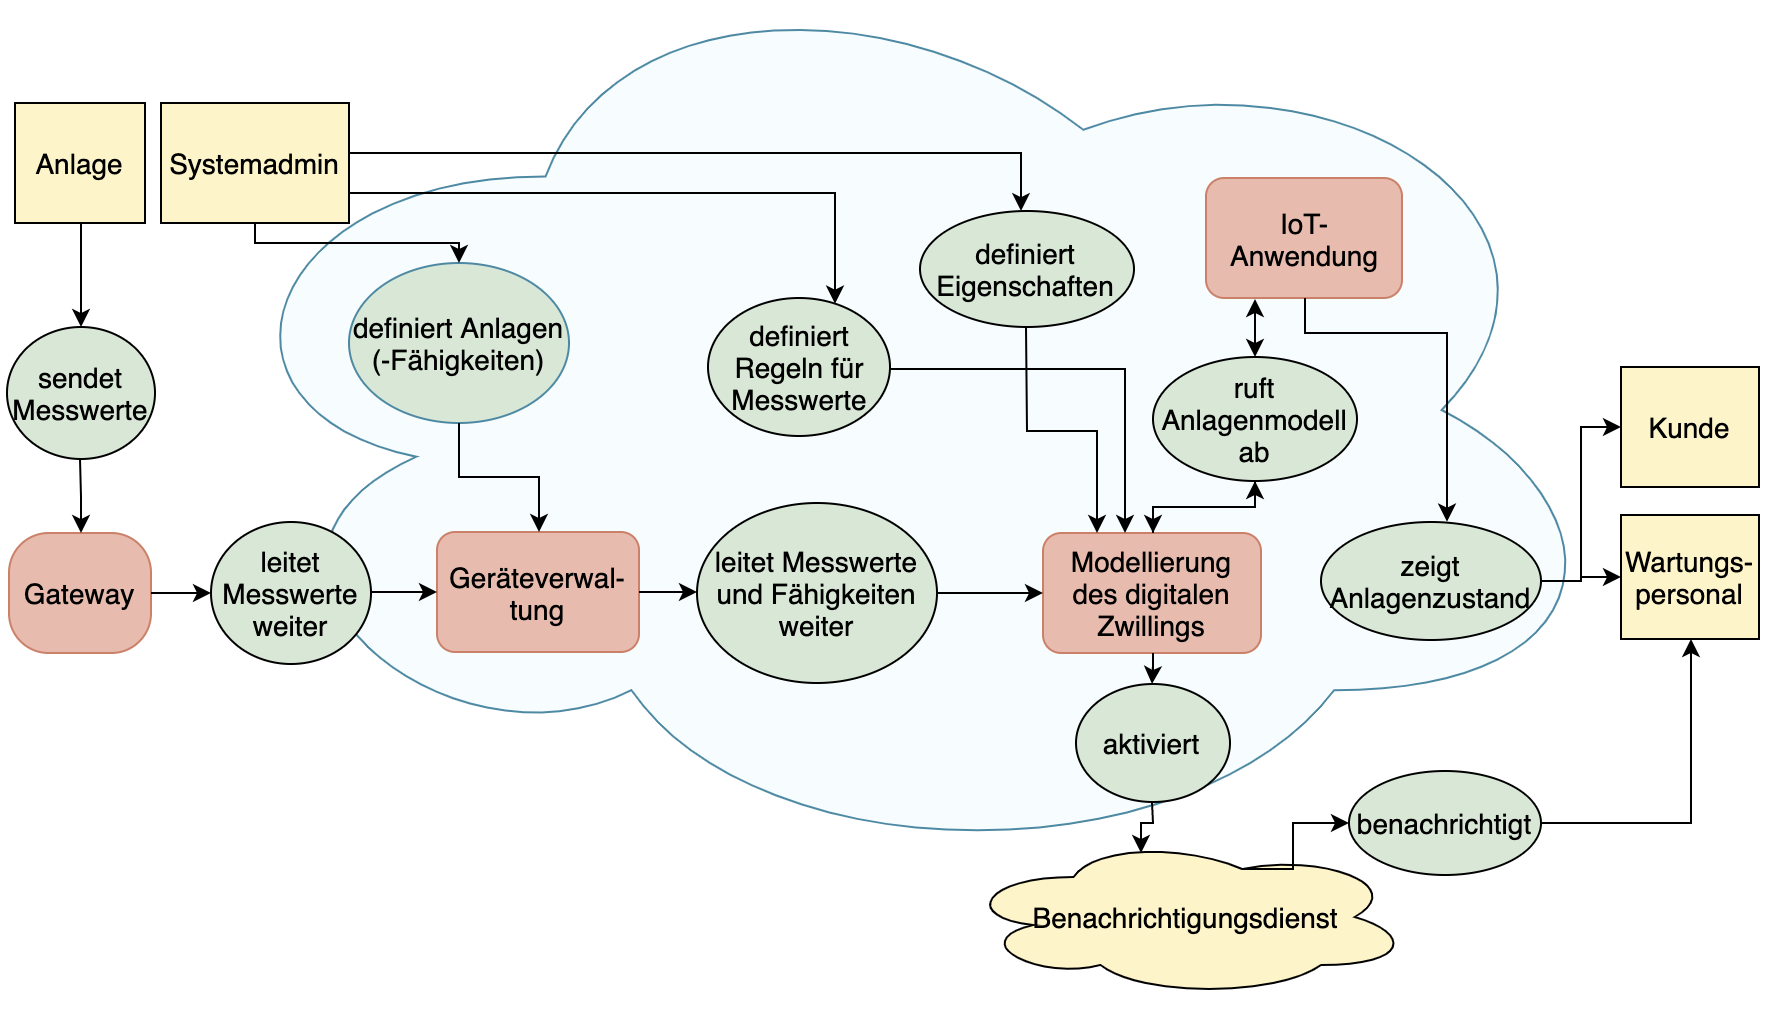
\includegraphics[width=1.0 \linewidth]{data_flow.png}
  \caption[Datenflussdiagramm]{Datenflussdiagramm}
  \label{dataflow}
\end{figure}

\noindent Aus dem Diagramm sind die \textbf{Schnittstellen} Anlage, Systemadmin, die Nutzer und der Benachrichtigungsdienst zu entnehmen. Technisch gesehen existieren noch weitere Schnittstellen, über die Daten verarbeitet und ausgetauscht werden.

\begin{enumerate}
  \item \textit{Systemadmin} zur \textit{Cloud}: Der Systemadmin soll über Benutzerschnittstellen zur Geräteverwaltung Typen und Instanzen der Anlage definieren. Eine Anlage soll aus aus n Sensoren und einem Gateway bestehen.
  \item \textit{Sensoren} zur \textit{Anlage}: Sensoren sollen Windgeschwindkeit (km/h), Luftfeuchtigkeit (\%), Temperatur (°C), Luftdruck (hpA) und die Luftdichte ($m^3$) erfassen.
  \item \textit{Anlage} zur \textit{Cloud}: Messwerte sollen von der Anlage über ein \textit{Gateway} an die Zieladresse der Anlageninstanz in der Geräteverwaltung gesendet werden.
  \item \textit{Systemadmin} zum \textit{digitalen Zwilling}: Der Systemadmin soll über Programmierschnittstellen Anlagentypen und -instanzen für die Zwillinge erzeugen, damit sie in eine Anwendung integriert werden können. Außerdem sollen Regeln und Funktionen für die Anlagentypen definiert werden.
  \item \textit{Anlageninstanz} zum \textit{digitalen Zwilling}: Die Messwerte der Anlage sollen dem digitalen Zwilling übergeben werden.
  \item \textit{Benachrichtigungsdienst} zum \textit{digitalen Zwilling}: Der Benachrichtigungsdienst soll über die definierten Regeln für die Anlage aktiviert werden.
  \item \textit{Nutzer} zur \textit{Anwendung}: Die Nutzer sollen die Anlagen über eine grafische Benutzerschnittstelle einsehen können.
  \item \textit{optional: Digitaler Zwilling} zur \textit{Anlage}: Der digitale Zwilling soll Befehle an die Anlage senden.
\end{enumerate}

% Use Cases
\paragraph{Anwendungsfälle}

Damit die Anwendungsfälle der Nutzer erfüllt werden können, müssen innerhalb des Systems neue Anwendungsfälle behandelt werden. Die neuen Fälle betreffen die Funktionen, die der Systemadministrator ausführen muss, damit die physische Anlage und dessen Daten virtuell repräsentiert werden können. In Abbildung \ref{usecasediagram} werden die neu ermittelten Anwendungsfälle in einem neuen Use Case Diagramm dargestellt.

\begin{figure}[ht!]
  \centering
  
\includegraphics[width=1.0\linewidth]{usecase_iot_prototype.png}
  \caption[Erweitertes Use Case Diagramm auf Systemebene]{Erweitertes Use Case Diagramm auf Systemebene}
  \label{usecasediagram}
\end{figure}
% Anforderungen Systemebene
\paragraph{Anforderungen}

Die Evaluation des Lösungsmodells mit dem Anwendungsfalldiagramm und dem Datenflussdiagramm ergibt die wesentlichen Teilsysteme des geplanten Systems. Die funktionale Anforderungsdefinition bezieht sich demnach auf die Teilbereiche, die ein Gesamtsystem ergeben (s. Anhang \ref{anf_system}):
\begin{enumerate}
  \item \textit{Das Messinstrument zur Simulation einer Anlage} (S-FA-1) muss min. alle 5 Sekunden die Daten erfassen, verarbeiten und direkt an die Geräteverwaltung senden können.
  \item \textit{Die Integration und Virtualisierung der Anlage} (S-FA-2) einschließlich der Behandlung der Anwendungsfälle muss durch den Prototyp gewährleistet werden.
  \item \textit{Die Visualisierung der Anlage} (S-FA-3) muss durch eine Benutzerschnittstelle für die Nutzer gewährleistet werden.
\end{enumerate}

\noindent Die detaillierte Definition der Anforderungen an Teilfunktionalitäten und an die Qualität und Sicherheit ist der Tabelle aus dem Anhang \ref{anf_system} zu entnehmen.

% Technische Ebene
\subsubsection{Technische Ebene}
Im Kapitel der Systemebene wurde logisch beschrieben, was der Prototyp können soll und über welche Schnittstellen diese Ziele erreicht werden sollen. Allerdings wurde noch nicht beschrieben, welche technischen Anforderungen sich für die Erreichung der Ziele ergeben.

\paragraph{Problemstellungen}

Damit das System nach dem vorgestellten Aufbau realisiert werden kann, muss das  technische System bestimmte Probleme lösen:

  \begin{tabularx}{\textwidth}{@{}lXp{2cm}@{}}
      \toprule
      ID                & Problem & Quelle \\
      \midrule
      \endhead
      \textbf{T-P-1}              &       Erzeugung eines cyber-physischen Systems als Messinstrument für die Anlagensimulation                       \\
      \multicolumn{1}{r}{T-P-1.1} & Lokale Verarbeitung der Messwerte  & \textit{S-FA-1}  \\
      \multicolumn{1}{r}{T-P-1.1} & Kommunikation zwischen Anlage und Geräteverwaltung  \\
      \textbf{T-P-2}              &    Übergabe in die digitale Welt    & \textit{S-FA-2} \\
      \multicolumn{1}{r}{T-P-2.1}              &       Einheitliche Kommunikation im Gesamtsystem      \\
      \multicolumn{1}{r}{T-P-2.2}              &  Adressierbarkeit aller Komponenten \\
      \multicolumn{1}{r}{T-P-2.3} & Erzeugung eines digitalen Zwillings \\
      \multicolumn{1}{r}{T-P-2.4} & Datentransfer zum digitalen Zwilling \\
      \multicolumn{1}{r}{T-P-2.5} & Kategorisierung der Messwerte \\
      \multicolumn{1}{r}{T-P-2.6} & Generierung von Events \\
      \textbf{T-P-3}              &  Einbindung eines externen Benachrichtigungsdienstes &\textit{S-FA-2}\\
      \textbf{T-P-4}              &  Erzeugung einer Anwendung zur Visualisierung & \textit{S-FA-3}\\
      \multicolumn{1}{r}{T-P-4.1} & Hardware- und ortsunabhängige Verfügbarkeit der Informationen  \\
      \textbf{T-P-5}              &  Sicherheit der Informationen & \textit{S-QA-3}\\
      \addlinespace
      \bottomrule
      \caption{Probleme aus technischer Ebene}
      \label{technik_probleme}
  \end{tabularx}



% Lösung aus technischer Ebene
\paragraph{Technischer Aufbau des Systems} \label{technischeraufbau}

Für die Simulation einer Windenergieanlage wird ein kommunikationsfähiges System benötigt, welches Schnittstellen für Sensoren als Messmittel aufweist (T-P-1). Mit der Nutzung eines \textit{Raspberry Pi 3 Model B} können durch die lokale Nutzung von Python-Skripten die Messwerte verarbeitet werden. Anschließend können die Messwerte durch die Anwendung des REST-Paradigmas über ein Gateway an die SAP Cloud Platform gesendet werden. Die weiteren Probleme werden durch die Nutzung der SAP"=Leonardo"=Technologien gelöst. Diese werden im nachfolgenden Kapitel detaillierter analysiert. Daher wird der technische Aufbau im Detail in dem nachfolgenden Kapitel vorgestellt. Technisch soll das System dem Paradigma des Cloud-Computing, also der Nutzung von Microservices, folgen.

\paragraph{Anforderungen}\label{anftechnik} Die technische Umsetzung des Prototypen muss folgenden Anforderungen folgen:

  \begin{tabularx}{\textwidth}{@{}lXp{1.5cm}@{}}
      \toprule
      ID                & Anforderung & Quelle \\
      \midrule
      \endhead
      \textbf{T-FA-1}              &    Die Simulation muss hardwareseitig rechnergestützt sein.       & \textit{T-P-1}                \\
      \multicolumn{1}{r}{T-FA-1.1} &   Die Hardware muss Schnittstellen zur Sensoreinbindung aufweisen. \\
      \multicolumn{1}{r}{T-FA-1.1} &   Die Software muss fähig sein, Berechnungen mit den empfangenen Sensorwerten zu durchzuführen. \\
      \multicolumn{1}{r}{T-FA-1.1} &   Die Software muss fähig sein, Messwerte über eine REST-API an ein Gateway zu versenden. \\
      \textbf{T-FA-2}              &   Das Gateway muss fähig sein, die Messwerte zu empfangen.   \\
      \multicolumn{1}{r}{T-FA-2.1}     &   Das Gateway muss fähig sein, die empfangenen Daten über eine REST-API zu versenden.   \\
      \multicolumn{1}{r}{T-FA-2.2} & Das Gateway kann fähig sein, die erfassten Daten vor dem Versenden zu verarbeiten. \\
      \multicolumn{1}{r}{T-FA-2.3} & Das Gateway muss fähig sein, Befehle aus der SAP Cloud Platform zu empfangen. \\
      \textbf{T-FA-3}            &      Der Prototyp muss fähig sein, die Messwerte vom Gateway zu empfangen. &    \textit{T-P-2}    \\
      \multicolumn{1}{r}{T-FA-3.1}    &  Der Prototyp muss fähig sein, die Messwerte einer eindeutigen \textit{DeviceId} zuzuordnen. \\
      \multicolumn{1}{r}{T-FA-3.2}    &  Der Prototyp muss fähig sein, der \textit{DeviceId} eine eindeutige \textit{GatewayId} zuzuordnen. \\
      \multicolumn{1}{r}{T-FA-3.3}    &  Der Prototyp muss fähig sein, die Messwerte einer \textit{DeviceId} an einen digitalen Zwilling zu übergeben.\\
      \multicolumn{1}{r}{T-FA-3.4}    &  Der Prototyp muss fähig sein, die Metadaten einer \textit{DeviceId} an einen digitalen Zwilling zu übergeben. \\
      \multicolumn{1}{r}{T-FA-3.5}  &  Der Prototyp muss fähig sein, Messwerte als \textit{High, Medium, Low} zu kategorisieren. \\
      \multicolumn{1}{r}{T-FA-3.6}  &  Der Prototyp muss fähig sein, automatisch POST-Anfragen an die Web-API eines \ac{sns} zu senden.  \\
      \textbf{T-R-1} & Der Prototyp muss die digitalen Zwillinge in einer UI5-Web-Applikation visualisieren. \\
      \textbf{T-R-2} & Der Prototyp und zugehörige Daten müssen in der SAP Cloud Platform gehosted sein.  \\
      \addlinespace
      \bottomrule
      \caption{Anforderungen aus technischer Ebene}
      \label{technik_anforderung}
  \end{tabularx}

  \newpage


